\section{RITAS algorithm}

Our algorithm constructs yield maps through the following steps:
Rectangle creation, Intersection assignment, Tesselation,
Apportioning, and Smoothing (RITAS). The overarching goal of this
process is to mimic the real world harvesting processes. Figure
\ref{fig:closeup} provides an illustration of these steps.

\begin{figure}[h!]  \centering
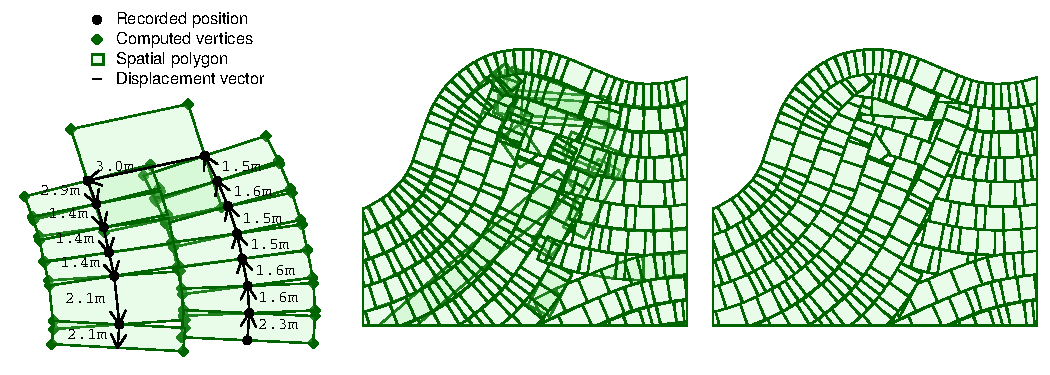
\includegraphics[width=\textwidth]{algoplots}
    \caption{Close-up illustration of some of the pre-processing
steps. \underline{Left}: construction of the vehicle polygons from the
GPS location data. Black dots mark the location at the end of each
logging cycle, green dots correspond to the vertices computed
according to the displacement vector implied by two consecutive
spatial points. The distance traveled could be reported by the yield
monitor or estimated from the vector length. \underline{Center}:
spatial polygons reveal overlap (darker areas) due to driving
maneuvers. \underline{Right}: clipping eliminates the overlap by
assigning intersecting areas to the first polygon in time.}
    \label{fig:closeup}
\end{figure} \TODO{FIGURE 1: Replace with the version JN sketched,
scanned, and emailed.}

Each precision yield data set is assumed to have time-ordered rows
containing the following information: mass harvested $m_t$,
2-dimensional spatial coordinate $(x_t,y_t)$, and swath width $2w_t$
(so that $w_t$ represents the half-width) for $t=0,\ldots,T$.  We
assume any lag time has been effectively pre-processed by
appropriately matching the mass harvested to its 2-dimensional
location.  \JN{Add reference to techniques to do this.}

\paragraph*{Step 1: Rectangle creation}

Figure \ref{} illustrates the construction of a rectangular polygon
representing the harvested area between each sequential pair of
spatial coordinates.

The position vector $\mathbf{s_t} = (x_{t}, y_{t})$ represents the
location of the tracked device in a 2-dimensional plane at the time
step $t$, which we assume to be the midpoint of the combine harvester
head. The rectangle is then uniquely identified by the position of its
four vertices, two representing the beginning of the harvested area at
time step $t-1$ and two representing the end of the harvested area at
time step $t$. The linear displacement vector is equal to the vector
difference between the position vectors at two subsequent time steps
$\mathbf{s_t} - \mathbf{s_{t-1}}$. The first two vertices are computed
as the endpoints of a line segment perpendicular to the displacement
vector with midpoint at $\mathbf{s_{t-1}}$ and length equal to the
swath width. The remaining two vertices are found using the same
procedure but pivoting on the midpoint $\mathbf{s_t}$. The rectangle
associated with mass $m_t$ has these vertices \TODO{add four
  coordinates like in the following expression}:
$\{(x_{t-1} + d_t, y_{t-1} + d_ts'_t),(x_{t-1} - d_t, y_{t-1} -
d_ts'_t), (x_{t } + d_t, y_{t } + d_ts'_t),(x_{t } + d_t, y_{t } +
d_ts'_t)\}$ where $d_t = tan^{-1}(s'_t)$.

The measurement unit of the header width, typically reported in meters
or feet, and the coordinate reference system should be homogenized
appropriately. As the first spatial point has no displacement, this
processing yields $T$ rectangles with vertices collected in the set
$\mathcal{P} = \{P_{\tau}$: $\tau \in \{2, \dots, T\}\}$.

\paragraph{Step 2: Intersection assignment.}  Figure \ref{} shows end
result of this rectangle construction which produces rectangles will
overlap, an area called the \emph{intersection}, due to adjacent
harvester paths.

\OUTLINE{Motivate clipping} Geometries in $\mathcal{P}$ represent the
area over which the combine harvester passed, which may differ from
the effectively harvested area at each time step. Yield monitors allow
the operator to dynamically record the proportion of the header being
full of crop, yet the operator may not make adjustments consistently
and accurately. More expensive gear includes sensing equipment for
assessing crop width automatically. The header may not be full of crop
when harvesting the field boundaries (e.g. on outer edges, around
voids), or within them. The first pattern can be identified by visual
inspection as long strips of indicated low yield running along the
length of the field \cite{Blackmore1999}. Several algorithms for this
first kind of harvesting dynamics, which is beyond the scope of our
algorithm, have been proposed.

\OUTLINE{Motivate clipping cont'd} In the second case, as a byproduct
of the destructive sampling scheme, the discrepancy is linked to the
spatial superposition of the observational units that arise due to
local harvesting dynamics such as turns, wedges, parallel lines, and
traveling over harvested areas. Globally within a field, this
phenomenon can be exacerbated by factors such as field
characteristics, or narrow row crops (e.g. wheat). Generally,
overlapping cannot be assumed symmetrical nor time-invariant. For
example, pivoting motions overlap on the inner side and the proportion
of duplicated area varies at each time step depending on factors such
as the sharpness of the turns, the angle of the wedges, or the
obstacles faced by the operator.

\OUTLINE{Explain clipping} As a general framework to model the
time-varying effectively harvested area, we run a time-ordered
apportioning procedure over the rectangles in $\mathcal{P}$. Let
$\tilde{P}_\tau = P_\tau \setminus \left( \bigcup_{i = 2}^{\tau - 1}
P_i \right)$ be the time-ordered relative complement of the previously
harvested area in the rectangle corresponding to the time step $t$. By
doing this, we effectively map the set of overlapping rectangles
$\mathcal{P}$ into a set of non-overlapping polygons
$\tilde{\mathcal{P}} = \{\tilde{P}_{\tau}: \tau \in \{2, \dots, T
\}$. When the original dataset has no voids (e.g. unplanted, flooded,
or more generally inaccessible sub areas), $\tilde{\mathcal{P}}$ form
a flat plane covered by tiles with no overlaps and no gaps
(non-periodic tessellation). Some of the computational considerations
discussed in \cite{Drummond1999} are relevant for implementing this
step.

This step creates $T$ polygons which partition the harvested area.
Each polygon is associated with the same mass it had in Step 1, but
now the area may be smaller (due to the intersection removal) and thus
yield is more accurately captured.

\paragraph*{Step 3: Tessellation and Apportioning} \OUTLINE{Motivate
gridding \& apportioning} The elements in $\tilde{\mathcal{P}}$ are
unsuitable for spatial techniques that do not accomodate to areas with
irregular shapes and heterogeneous area sizes. Two equally-sized long
rectangles, one in a vertical and the other in a horizontal position,
would have the same centroid yet they convey different information
about yield to the north or west of the centroids. Alternatively, two
centered equally-shaped polygons with different sizes carry different
information about the spatial coverage of the collected data. To
normalize the aerial representation in terms of both shape and size,
we superimpose a regular grid of square pixels, assign portions of the
polygons into grid pixels, and apportion the harvested mass associated
with the polygons to the pixels. The first two steps involve topology
operations on geometries whereas the last one involves manipulation of
the numerical data. Accounting for these two spatial features is by
itself a methodological improvement over the surveyed algorithms,
which simply reduce data to spatial points such as the displacement
vector endpoint or, less commonly, the polygon centroid.

\OUTLINE{Explain gridding \& apportioning} Let $\mathcal{P}^{*}_N$ be
a set of $N \in \mathbb{N}$ equally-sized, non-overlapping, and
contiguous squared pixels forming a grid covering all the elements in
$\tilde{\mathcal{P}}$. The constant $N$ reflects the preference of the
map user in terms of resolution, selected either by the total number
of pixels, more intuitively by the pixel length in meters, or the
target computational time investment. Although pixels size can be set
arbitrarily, its choice should consider the accuracy of the position
system. We take the pairwise intersection among the elements in
$\tilde{\mathcal{P}}$ and $\mathcal{P}^{*}_N$ and compute $\pi_{\tau,
n} \in [0, 1]$ the proportion of the area in the $\tau$-th
non-overlapping polygon $P_{\tau}$ that intersects with the $n$-th
pixel in the grid for $\tau \in \{2, \dots, T\}$ and $n \in \{1,
\dots, N\}$. The corresponding proportion of the harvested mass
$m_{\tau}$ associated with $P_{\tau}$ is assigned to $P^{*}_N$. The
total harvested mass associated with the $n$-th pixel is given by
$m^{*}_n = \sum_{\tau = 2}^{T} \pi_{\tau, n} \ m_{\tau}$. The
resulting polygons in $\mathcal{P}^{*}_N$ resemble much the Basic
Areal Units (BAUs) as defined by \cite{Nguyen2012} in the context of
massive data fusion: fine-scale, nonoverlapping, aereal regions
representing the smallest resolution at which data is aggregated.

\OUTLINE{Apportioning key fact (1)} Two key aspects behind the
gridding strategy are worth mentioning. First, for the purpose of
apportioning, we assume that the harvested mass associated with the
spatial polygons is distributed uniformly within each unit. This is a
sensible assumption in this context as combine harvester log data in
short cycles and the spatial polygons represent small areas for the
scale of the underlying crop growth process.

\OUTLINE{Apportioning key fact (2)} Second, if one imposes regularity
and equal-shape conditions on the grid elements and also forces it to
cover all the elements in $\tilde{\mathcal{P}}_{\tau}$, the sum of the
pixels area may exceed the sum of the tessellated polygons area. The
excess, found at both the harvested region outer borders and the inner
voids boundaries, can be diagnosed visually with ease. It decreases as
the grid resolution, or equivalent as the total number of pixels $N$,
increases and so can be controlled at the cost of additional
computational time for topology operations and smoothing. %More
Concretely, when a Gaussian Process is applied for smoothing as
described below, exact inference has time complexity in the order of
$O(N^3)$ and storage demands of of $O(N^2)$. In other words, as we
double the map resolution, we octuple the number of operations and
quadruple the need for storage.  Alternatively, one could exclude the
pixels with less than an arbitrary proportion of area effectively
covered by the tessellated observations. A sensible choice, such as a
minimum coverage of 50\%, will tend to balance under and over-covered
polygons. Due care should be taken so that apportioning is still
applied validly: mass should be allocated to pixels only in proportion
of the actual overlapping area, discarding any part of the tessellated
polygons that is not covered by any pixel. Note that the grid
resolution serves only for the purpose of spatial aggregation, and
need not be the same resolution used for the visualization that will
be introduced in the following step.

Mass is apportioned from the polygons of Step 2 to tiles in the
grid according to their proportion of the total polygon
area. Where tiles overlap multiple polygons, the tiles receive mass
from each of the polygons according to the area of overlap relative to
each polygon's area.  Thus, the mass associated with the $n$th tile is
$m_n^* = \sum_{t=1}^T p_{t,n} m_t$ where $p_{t,n}$ is the proportion
of polygon $t$'s area in the intersection of polygon $t$ and tile $n$.
This step creates $N$ polygons, determined by the user based on
tesselation resolution, partitioning the harvested area each with an
associated mass of harvested crop.

\paragraph{Step 4: Smoothing} Figure \ref{} shows the regular
tesselation with apportioned mass.  The regular tesselation provides
constant areas and meaningful centroids, and therefore we can use
standard spatial smoothing techniques directly on mass, as opposed to
yield. \cite{McCullagh2006} provided empirical evidence suggesting
that the non-anthropogenic spatial variation in yield, defined as
patterns that cannot be explained by topography or human intervention,
matches the characteristics of the de Wijs process plus white
noise. We smooth using a Gaussian Process (GP) with a Mat\'ern
covariance on the logarithm of mass
\citep{handcock1993bayesian,gutt2006studies}. Compared with the more
common powered exponential covariance functions, e.g. Gaussian or
exponential, the Mat\'ern adds an additional parameter that controls
local smoothness, i.e. \ differentiability, and therefore is often
more accurate for real world processes.

Covariance parameters are estimated, and smoothed values are found for
each tile following \cite{Cressie1993}.  Specifically, for each tile
we have a predicted mean $\hat\mu_{\ell}$ and variance
$\hat\sigma^2_{\ell}$ for the logarithm of mass.  We using the
following formulas to convert back to the mean and variance of mass
\[ \hat{\mu}_{m} = \exp\left(\hat{\mu}_{\ell} +
\hat{\sigma}^2_{\ell}/2\right), \quad\mbox{and}\quad
\hat{\sigma}^2_{m} = \exp\left(2 \hat{\mu}_{\ell} +
\hat{\sigma}^2_{\ell}\right)
\left[\exp\left(\hat{\sigma}^2_{\ell}\right) - 1\right].
 \] Finally, yield is calculated by dividing the tile mass by the tile
area.  Figure \ref{} provides smoothed version of Figure \ref{}.

\subsection{Protocol assessment}

One appealling aspect of our approach is that data are not eliminated
based on arbitrary thresholds.

\JN{What percentage of observations did we throw out?  Vega used R,
can we compare to running his algorithm on our data.}

\JN{Variogram}

\LD{Correlation Yield, TWI for YM raw data vs aggregated vs smoothed}

%%% Local Variables:
%%% mode: latex
%%% TeX-master: "../thesis"
%%% End:
